\documentclass[conference]{IEEEtran}
\usepackage{cite}
\usepackage{amsmath,amssymb,amsfonts}
\usepackage{graphicx}
\usepackage{booktabs}
\usepackage{multirow}
\usepackage{url}
\usepackage{float}
\usepackage{xcolor}
\usepackage{placeins}
\usepackage{tikz}
\usetikzlibrary{arrows.meta, positioning, shapes.geometric, fit, calc}

\begin{document}

\title{Mayalok: From a Smartphone Walkthrough to a Searchable Gaussian-Splat Digital Twin with Obstacle-Aware Browser Navigation}

\author{
\IEEEauthorblockN{
Ajay Yadav\textsuperscript{1},
Hitesh Bhatiwal\textsuperscript{2},
and Harsh Vardhan\textsuperscript{3}
}
\IEEEauthorblockA{
Team QWERTY (Team ID TM-E434D6B6C8) \\
Techfest 2026--27, Namma Space Challenge, IIT Bombay \\
\textsuperscript{1}Team leader \\
Code and live demo: \url{https://github.com/The-Harsh-Vardhan/mayalok}, \url{https://mayalok.vercel.app}
}
}

\maketitle

\begin{abstract}
Digital twins of indoor venues are usually built with LiDAR scanners or CAD models, which most small venues cannot afford. This paper presents Mayalok (formerly Namma Space), an open pipeline and web viewer that turns ordinary smartphone video into a photorealistic 3D Gaussian Splat of an indoor space and serves it as a zero-install first-person walkthrough with place search and obstacle-aware walking directions. An offline, resumable Python pipeline extracts sharp keyframes, recovers camera poses with COLMAP-family structure-from-motion, fixes gravity, floor and metric scale (ArUco markers or a fixed phone-height rule), trains a 3D Gaussian Splatting model, removes floaters, and derives a 5~cm occupancy grid. The viewer renders the compressed \texttt{.spz} splat with Spark.js on Three.js, indexes places with Fuse.js, and plans routes with A* in a Web Worker over the same grid. We report two real runs on one incubation-centre capture. A single 56.8~s video produced 293 keyframes, of which 65 registered (6,660 sparse points, 0.52~px mean reprojection error); Brush trained 430,487 Gaussians, 191,378 of which survived cleaning, giving a 4.7~MB \texttt{scene.spz} and a 2.66~m\textsuperscript{2} walkable area after agent-radius tuning. A second run over all 603 captured images registered 523 images in one GLOMAP model at 0.72~px, but the resulting splat showed cross-clip misalignment and was excluded. We present these results as a feasibility study, state what was not measured, and describe the limitations that follow.
\end{abstract}

\begin{IEEEkeywords}
3D Gaussian Splatting, structure from motion, indoor digital twin, occupancy grid, A* pathfinding, web rendering, smartphone capture.
\end{IEEEkeywords}

\section{Introduction}
Indoor navigation aids for campuses, incubators, exhibitions, and small commercial venues depend on an accurate digital model of the space. Building such a model with terrestrial laser scanners or hand-authored CAD floor plans is slow and expensive, and the result is rarely photorealistic. At the same time, modern phones record sharp high-resolution video, and neural scene representations can turn such video into a navigable 3D scene. Neural Radiance Fields (NeRF) made photorealistic novel-view synthesis from posed images practical \cite{mildenhall2020nerf,barron2022mipnerf360}, and 3D Gaussian Splatting (3DGS) added real-time rendering by representing a scene as millions of anisotropic Gaussians that are rasterized and alpha-blended \cite{kerbl2023}. The gap that remains is not reconstruction quality alone. A visitor needs a scene that loads in a browser, uses true metric units, can be searched for named places, and supports walking directions that respect walls and furniture.

Mayalok addresses that gap as an end-to-end system. It combines an offline reconstruction pipeline with a static web viewer, and it derives both collision and routing from a single 2D walkable grid computed from the splat itself. The central design decision is to treat that grid as the one spatial index shared by collision, pathfinding, and a future augmented-reality layer. A second decision is to keep every pipeline stage a plain-file transformation, so a stage can be re-run, tuned, or swapped without recomputing earlier ones.

This report documents the design and the evidence behind it. We deliberately limit the scope to what the repository implements and what was measured on one real capture: an incubation centre recorded on 24~Oct~2026 for the Techfest 2026--27 Namma Space challenge. We do not claim a benchmark against other capture systems, a user study, or sub-centimetre accuracy, and where the reference-style sections of a measurement paper would call for such results we instead state the method, the limitation, and the planned work.

\subsection{Contributions}
The main contributions are as follows:
\begin{itemize}
    \item We present an open, resumable smartphone-to-splat pipeline with eight stages (frames, SfM, alignment, training, cleaning, navigation grid, export, viewer) and a metric, floor-at-zero, $+Y$-up world frame shared by every later stage.
    \item We describe a single-grid design in which a 5~cm occupancy grid derived from the cleaned splat drives collision, A* routing with wall-aware cost, path smoothing, and turn-by-turn instructions in a browser Web Worker.
    \item We report two real reconstruction runs of the same venue with exact counts, including a single-video run that produced a usable but partial scene and a multi-clip run that registered most images yet failed visually, and we analyze why low reprojection error was not sufficient evidence of a usable splat.
    \item We release the system as an MIT-licensed repository, a live demo, and a Python package (\texttt{pip install mayalok}, PyPI release 0.1.0) \cite{mayalokrepo}.
\end{itemize}

\section{Related Work}
\subsection{Novel-View Synthesis and Gaussian Splatting}
NeRF represents a scene as a neural field queried along camera rays and optimized from posed images \cite{mildenhall2020nerf}. Mip-NeRF~360 extended this to unbounded real scenes with anti-aliased sampling and established a widely used benchmark of indoor and outdoor captures \cite{barron2022mipnerf360}. 3DGS replaced the implicit field with an explicit set of Gaussians whose means, covariances, opacities, and view-dependent colors are optimized, and rendered them with a tile-based differentiable rasterizer at interactive rates \cite{kerbl2023}. Each Gaussian is
\begin{equation}
G(\mathbf{x}) = \exp\!\left(-\tfrac{1}{2}(\mathbf{x}-\boldsymbol{\mu})^{\top}\boldsymbol{\Sigma}^{-1}(\mathbf{x}-\boldsymbol{\mu})\right), \quad \boldsymbol{\Sigma}=\mathbf{R}\mathbf{S}\mathbf{S}^{\top}\mathbf{R}^{\top},
\end{equation}
and a pixel color is the front-to-back blend
\begin{equation}
C(\mathbf{p}) = \sum_{i \in \mathcal{N}} \mathbf{c}_i \,\alpha_i \prod_{j<i}\left(1-\alpha_j\right).
\end{equation}
Densification strategy and Gaussian count matter for deployment. A Markov-chain Monte Carlo formulation of densification allows a hard cap on the number of Gaussians, which bounds memory and download size \cite{kheradmand2024mcmc}. The open-source library gsplat packages efficient 3DGS training with this strategy \cite{ye2024gsplat}, and Brush provides a cross-platform trainer \cite{brush}. Mayalok uses both: gsplat is the default trainer and Brush is the fallback on machines where gsplat does not build.

\subsection{Structure from Motion}
3DGS needs camera poses, which are typically obtained with structure from motion. COLMAP is the standard incremental pipeline, built on SIFT features \cite{lowe2004sift} and robust geometric verification \cite{schonberger2016sfm}. Incremental mapping is accurate but slow and can fragment a capture into several sub-models. Global SfM, in particular GLOMAP, estimates all poses jointly and is much faster on large unordered sets \cite{pan2024glomap}. Our pipeline uses the global mapper first and falls back to incremental mapping if too few frames register. The multi-view geometry underlying triangulation of markers and sparse points follows standard treatments \cite{hartley2004mvg}.

\subsection{Metric Scale, Fiducials, and Orientation}
Monocular SfM recovers geometry only up to a similarity transform. A routing system needs true meters, so we recover scale from printed square fiducial markers detected with ArUco \cite{garridojurado2014aruco} or, when none are visible, from a fixed phone height. Gravity direction comes from camera orientations, the floor plane from a RANSAC fit \cite{fischler1981ransac}, and in-plane rotation from a Manhattan-world assumption that walls align with two orthogonal axes \cite{coughlan1999manhattan}.

\subsection{Occupancy Grids and Pathfinding}
Occupancy grids discretize free space for planning. A* finds minimum-cost paths on such a graph with a consistent heuristic \cite{hart1968astar}. We use an 8-connected grid with octile distance, add a clearance-dependent step cost so routes centre themselves in corridors, and smooth the cell path by string pulling. The grid is computed with standard array and morphology routines \cite{virtanen2020scipy,bradski2000opencv}.

\subsection{Web Delivery of Splats}
Browser delivery needs a compact format and a GPU renderer. The SPZ format compresses Gaussian splats for transmission \cite{spz2025}, Spark.js renders splats inside Three.js scenes \cite{spark2025,threejs}, and splat-transform converts PLY files to SPZ \cite{splattransform}. For place lookup we use client-side fuzzy search \cite{fusejs}. Table~\ref{tab:positioning} positions Mayalok against these building blocks; it is a qualitative comparison of roles, not a performance comparison.

\begin{table*}[!tb]
\centering
\footnotesize
\caption{Positioning of Mayalok Against the Components It Builds On (Qualitative)}
\label{tab:positioning}
\begin{tabular}{p{0.17\textwidth}p{0.22\textwidth}p{0.25\textwidth}p{0.27\textwidth}}
\toprule
\textbf{Work} & \textbf{Representation} & \textbf{Contribution} & \textbf{Role in Mayalok} \\
\midrule
NeRF \cite{mildenhall2020nerf}, Mip-NeRF~360 \cite{barron2022mipnerf360} & Implicit radiance field & Photorealistic novel views; unbounded-scene benchmark & Motivation; not used, Mayalok adopts explicit splats instead \\
3DGS \cite{kerbl2023} & Explicit Gaussians & Real-time rasterized splat rendering & Core scene representation \\
3DGS-MCMC \cite{kheradmand2024mcmc}, gsplat \cite{ye2024gsplat} & Explicit Gaussians with capped count & Bounded Gaussian budget; training library & Default training path with 1.5M cap \\
COLMAP \cite{schonberger2016sfm}, GLOMAP \cite{pan2024glomap} & Sparse points and poses & Incremental and global SfM & Pose recovery and fallback \\
ArUco \cite{garridojurado2014aruco} & Square fiducials & Robust marker detection & Optional metric-scale source and AR anchors \\
SPZ \cite{spz2025}, Spark.js \cite{spark2025} & Compressed splat file, GPU renderer & Small downloads, in-browser rendering & Delivery and rendering layer \\
\textbf{Mayalok} & Splat plus 5~cm walkable grid and POI file & End-to-end capture, grid, search, and routing & Integrates the above into one resumable pipeline and static viewer \\
\bottomrule
\end{tabular}
\end{table*}

\section{Capture Data and Study Scope}
\subsection{Venue and Captures}
The quantitative evidence comes from one venue, an incubation centre, captured on 24~Oct~2026 with a smartphone. The Technical Abstract records the session as 8 videos and about 40 photos. Two reconstruction runs are reported. The \emph{single-video run} uses one 56.8~s portrait video. The \emph{all-captures run} uses 603 images, which are keyframes from 7 videos together with 32 photos. The single-video run used a laptop with an RTX~4050 GPU (6~GB); the hardware of the multi-clip run is not recorded here. Table~\ref{tab:dataset_scope} records the scope. This boundary matters because the paper does not claim results across venues, devices, or lighting conditions.

\begin{table}[!htb]
\centering
\footnotesize
\caption{Data and Study Scope}
\label{tab:dataset_scope}
\begin{tabular}{p{0.38\columnwidth}p{0.50\columnwidth}}
\toprule
\textbf{Item} & \textbf{Value} \\
\midrule
Venue & Incubation centre (one site) \\
Capture date & 24 Oct 2026 \\
Capture session & 8 videos, about 40 photos \\
Single-video run input & 1 portrait video, 56.8 s \\
All-captures run input & 603 images (7 videos + 32 photos) \\
Compute (single-video run) & Laptop, RTX 4050 (6 GB) \\
Metric scale source & Phone-height rule (1.35 m); no ArUco markers in this capture \\
Challenge & Techfest 2026--27, Namma Space, IIT Bombay \\
\bottomrule
\end{tabular}
\end{table}

\subsection{Pipeline Stage Inventory}
Table~\ref{tab:stages} lists the stages, the module that implements each, the method, and the durable output. Every stage reads and writes plain files, and the orchestrator skips a stage whose outputs already exist unless \texttt{--force} is given. This lets a failed or retuned stage resume without recomputing earlier ones.

\begin{table*}[!tb]
\centering
\footnotesize
\caption{Pipeline Stage Inventory}
\label{tab:stages}
\begin{tabular}{p{0.04\textwidth}p{0.13\textwidth}p{0.41\textwidth}p{0.30\textwidth}}
\toprule
\textbf{No.} & \textbf{Module} & \textbf{Method} & \textbf{Durable output} \\
\midrule
1 & \texttt{namma.frames} & Oversampled extraction, sharpest frame per window (variance of Laplacian), blur floor at 35\% of median & \texttt{images/<clip>/*.jpg}, \texttt{frames.json} \\
2 & \texttt{namma.sfm} & SIFT features, sequential matching (15 neighbours), global mapper with incremental fallback & \texttt{sparse/}, undistorted dataset \\
3 & \texttt{namma.align}, \texttt{namma.markers} & Gravity from cameras, RANSAC floor, scale from markers or phone height, Manhattan yaw & Metric \texttt{cameras.json}, \texttt{alignment.json} \\
4 & \texttt{namma.train} & 3DGS via gsplat (MCMC, 30k steps, 1.5M cap) or Brush fallback & Trained \texttt{point\_cloud.ply} \\
5 & \texttt{namma.clean} & Opacity, size, bounds and statistical-outlier filters; vertical floor refit & Cleaned splat \\
6 & \texttt{namma.navgrid} & 5 cm occupancy grid, distance transform, walked-path repair, largest component & \texttt{navgrid.json}, \texttt{minimap.png} \\
7 & \texttt{namma.export} & PLY to SPZ with splat-transform; scene manifest & \texttt{scene.spz}, \texttt{scene.json} \\
8 & Web viewer & React, Three.js, Spark.js; Fuse.js search; A* in a Web Worker & Static site \\
\bottomrule
\end{tabular}
\end{table*}

\section{Methodology}
\subsection{System Overview}
Mayalok has two halves. The offline half runs in Python and produces a self-contained scene folder (\texttt{scene.spz}, \texttt{scene.json}, \texttt{navgrid.json}, \texttt{minimap.png}, \texttt{pois.json}, \texttt{report.json}). The online half is a fully static site that loads that folder, renders the splat, and runs search and routing on the client. Figure~\ref{fig:architecture_tikz} presents the conceptual architecture, Fig.~\ref{fig:system_context} shows the system context, and Fig.~\ref{fig:pipeline_stages} the stage outputs.

\begin{figure*}[!tb]
\centering
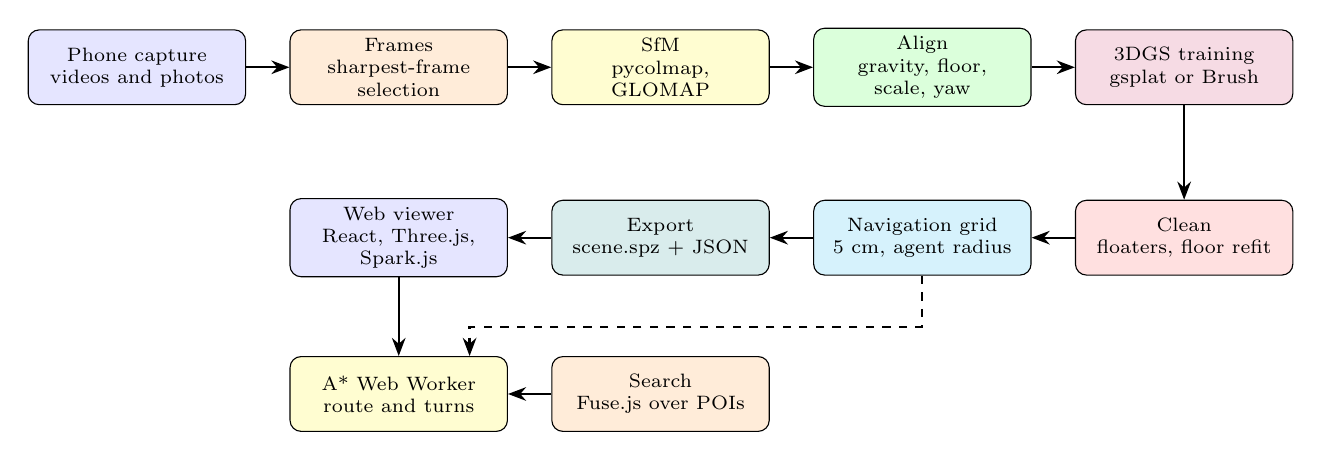
\begin{tikzpicture}[
    node distance=0.55cm,
    box/.style={
        draw,
        rounded corners,
        minimum height=0.95cm,
        text width=2.55cm,
        align=center,
        font=\scriptsize,
        inner sep=3pt
    },
    arrow/.style={-{Stealth[length=2.3mm]}, thick}
]
\node[box, fill=blue!10] (cap) {Phone capture\\videos and photos};
\node[box, fill=orange!15, right=of cap] (frames) {Frames\\sharpest-frame selection};
\node[box, fill=yellow!18, right=of frames] (sfm) {SfM\\pycolmap, GLOMAP};
\node[box, fill=green!14, right=of sfm] (align) {Align\\gravity, floor, scale, yaw};
\node[box, fill=purple!14, right=of align] (train) {3DGS training\\gsplat or Brush};
\node[box, fill=red!12, below=1.2cm of train] (clean) {Clean\\floaters, floor refit};
\node[box, fill=cyan!16, left=of clean] (grid) {Navigation grid\\5 cm, agent radius};
\node[box, fill=teal!15, left=of grid] (export) {Export\\scene.spz + JSON};
\node[box, fill=blue!10, left=of export] (viewer) {Web viewer\\React, Three.js, Spark.js};
\node[box, fill=yellow!18, below=1.0cm of viewer] (astar) {A* Web Worker\\route and turns};
\node[box, fill=orange!15, right=of astar] (search) {Search\\Fuse.js over POIs};
\draw[arrow] (cap) -- (frames);
\draw[arrow] (frames) -- (sfm);
\draw[arrow] (sfm) -- (align);
\draw[arrow] (align) -- (train);
\draw[arrow] (train) -- (clean);
\draw[arrow] (clean) -- (grid);
\draw[arrow] (grid) -- (export);
\draw[arrow] (export) -- (viewer);
\draw[arrow] (viewer) -- (astar);
\draw[arrow] (search) -- (astar);
\draw[arrow, dashed] (grid.south) |- ++(0,-0.65) -| ([xshift=0.9cm]astar.north);
\end{tikzpicture}
\caption{Conceptual architecture of Mayalok. The offline pipeline (top row, then right to left on the second row) produces a scene folder. The viewer loads it, and the navigation grid (dashed) is posted to a Web Worker that plans routes for searched places.}
\label{fig:architecture_tikz}
\end{figure*}

\begin{figure*}[!tb]
\centering
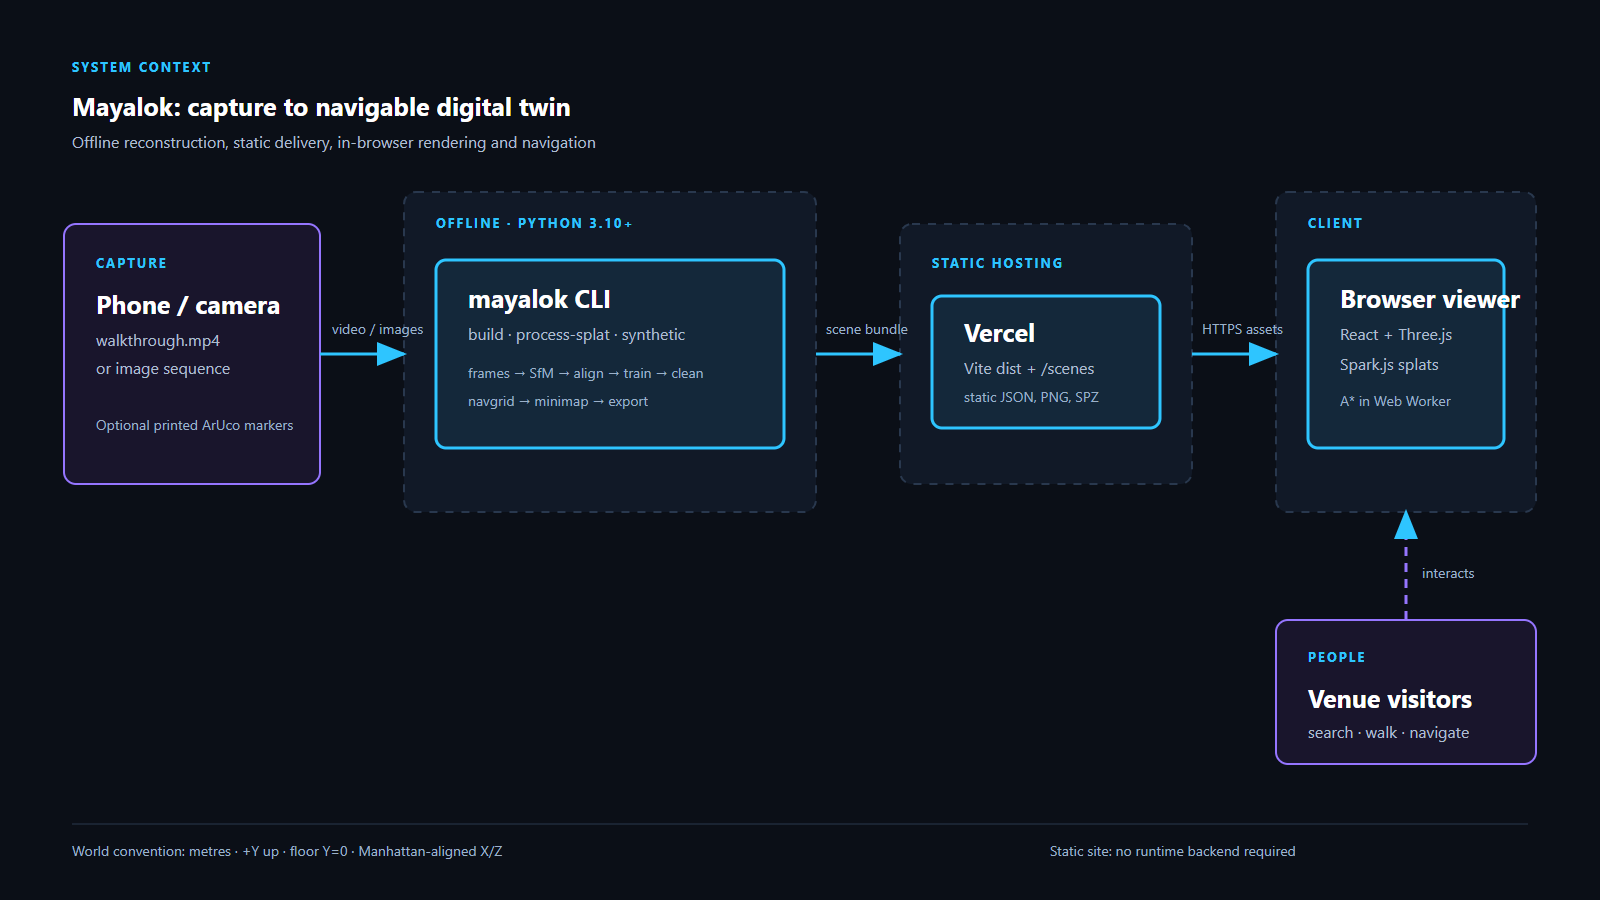
\includegraphics[width=0.92\textwidth]{figures/system-context.png}
\caption{System context from the repository diagrams: capture by phone, offline processing by the \texttt{mayalok} command-line tool, static hosting of the scene bundle, and the browser viewer used by venue visitors. The world convention is meters, $+Y$ up, floor at $Y=0$, Manhattan-aligned X/Z.}
\label{fig:system_context}
\end{figure*}

\begin{figure*}[!tb]
\centering
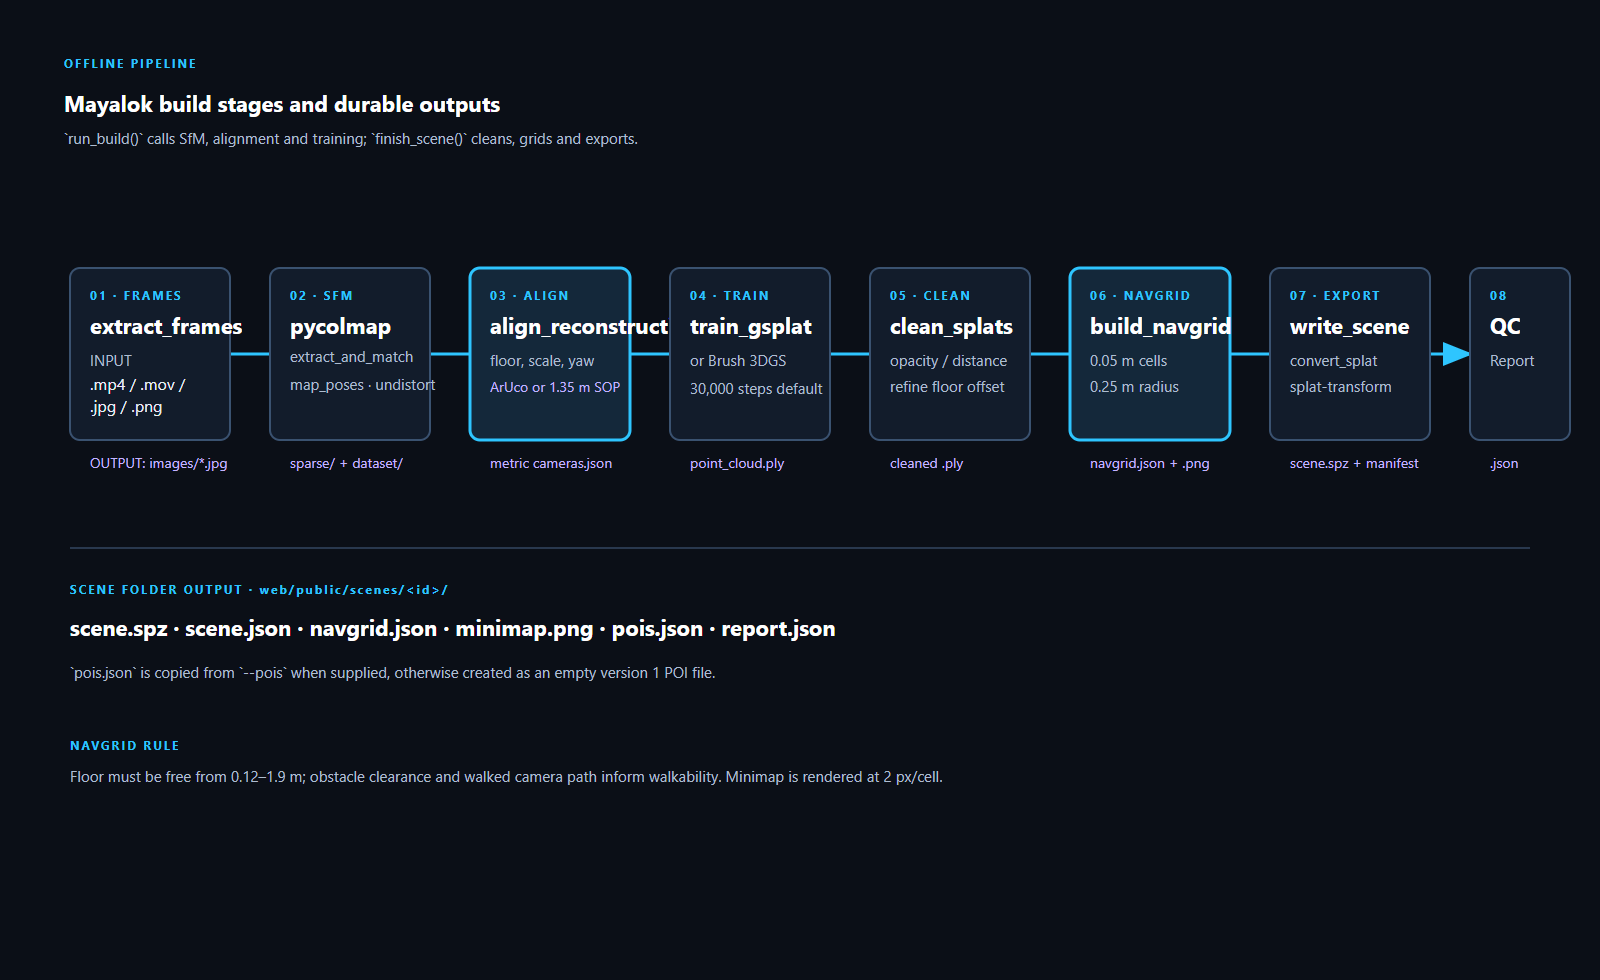
\includegraphics[width=0.92\textwidth]{figures/pipeline-stages.png}
\caption{Build stages and durable outputs. \texttt{run\_build()} runs frames, SfM, alignment, and training; \texttt{finish\_scene()} runs cleaning, the navigation grid, and export. The same tail also serves \texttt{process-splat}, which accepts an externally trained splat.}
\label{fig:pipeline_stages}
\end{figure*}

\subsection{Capture Protocol}
The capture standard operating procedure (SOP) is part of the method, because reconstruction quality is bounded by capture quality. The operator turns all lights on, clears floor clutter, closes unwanted doors, and avoids mirrors and glass. Scale comes from 3--4 printed ArUco markers (\texttt{DICT\_4X4\_50}, 15~cm side) taped flat on the floor, or from a constant phone height of 1.35~m. The operator walks slowly (about one step per second), covers the perimeter and then an inner pass, photographs corners and ceiling edges, keeps 60--70\% overlap, and walks the routes real visitors would use. One continuous clip suffices for a small space; a large space is split into one clip per zone with about 2~m of overlap. Capture takes about 3--5 minutes per room. The routes walked matter later, because the grid treats walked cells as free.

\subsection{Keyframe Extraction}
Videos are sampled at three times the target rate (default 2 keyframes per second after selection, long side capped at 1600~px). In each window only the sharpest frame is kept. Sharpness is the variance of the Laplacian of a downscaled grayscale copy,
\begin{equation}
S(I) = \operatorname{Var}\!\left(\nabla^{2} I\right),
\end{equation}
and a window is discarded if its best score is below 35\% of the median score over the clip. Photos are kept unless they are blurry. Each clip is written to its own folder so SfM can estimate separate intrinsics per clip. The single-video run used 5.5 keyframes per second at a 1024~px cap, which differs from the defaults and yielded 293 keyframes.

\subsection{Structure from Motion}
pycolmap extracts SIFT features (up to 8,192 per image) with a \texttt{SIMPLE\_RADIAL} camera model and one set of intrinsics per clip. Each frame is matched against its next 15 neighbours, with quadratic long-range jumps, and with optional vocabulary-tree loop detection. Poses come from COLMAP's global mapper (GLOMAP) \cite{pan2024glomap}. If the registered fraction falls below 70\%, the incremental mapper \cite{schonberger2016sfm} is also run and the larger model is kept. We report registration ratio $\rho = N_{\mathrm{reg}}/N_{\mathrm{img}}$ and mean reprojection error
\begin{equation}
\bar{e} = \frac{1}{|\mathcal{O}|}\sum_{(i,j)\in\mathcal{O}} \left\lVert \pi\!\left(\mathbf{K}_i,\mathbf{T}_i,\mathbf{X}_j\right) - \mathbf{x}_{ij} \right\rVert_2,
\end{equation}
where $\mathcal{O}$ is the set of observations, $\pi$ is the projection, and $\mathbf{x}_{ij}$ is the measured keypoint. Both quantities are standard but, as Section~\ref{sec:results} shows, neither certifies global consistency.

\subsection{Metric Scale, Gravity, Floor, and Yaw}
SfM output has arbitrary scale and orientation. The ``up'' direction is the negated mean of the cameras' downward axes, since full walking loops cancel forward and backward tilt. The floor is the lowest significant dense layer of sparse points below the median camera height, refined by RANSAC \cite{fischler1981ransac} with tilt limited to 10$^{\circ}$ and a least-squares refit on the inliers. Scale uses the first available source in the order manual override, ArUco markers, phone height. For markers, each marker (15~cm, up to 400 frames inspected) is triangulated by the direct linear transform \cite{hartley2004mvg} and accepted only with at least three views and low reprojection error; the scale is
\begin{equation}
s = \frac{\ell_{\mathrm{printed}}}{\operatorname{median}_m\left(\hat{\ell}_m\right)},
\end{equation}
with $\ell_{\mathrm{printed}}=0.15$~m and $\hat{\ell}_m$ the reconstructed side length of marker $m$. Without markers, the phone-height rule gives
\begin{equation}
s = \frac{h_0}{\tilde{h}_{\mathrm{cam}} - h_{\mathrm{floor}}},
\end{equation}
where $h_0 = 1.35$~m, $\tilde{h}_{\mathrm{cam}}$ is the median camera height along the up axis, and $h_{\mathrm{floor}}$ is the fitted floor height. Yaw is chosen to maximize the sum of squared histogram counts of wall points along the two horizontal axes over a 90$^{\circ}$ sweep, which aligns walls with the axes \cite{coughlan1999manhattan}. One similarity transform is applied to cameras and points, leaving the scene metric, $+Y$ up, floor at $Y=0$, with the origin at the centre of the walked area. The incubation scene used the phone-height rule.

\subsection{Gaussian Splat Training}
The trainer is gsplat's reference script \cite{ye2024gsplat} with MCMC densification \cite{kheradmand2024mcmc}, 30,000 steps by default, and a hard cap of 1.5 million Gaussians. World-space normalization is disabled so the metric frame is preserved, and every 8th frame is held out so the trainer can report held-out image quality. On Windows machines where gsplat does not build, Brush \cite{brush} is used instead. Both Mayalok runs reported here used Brush: 20,000 steps for the single-video run and 25,000 steps for the all-captures run. Held-out image-quality metrics such as PSNR and SSIM \cite{wang2004ssim} were not recorded for these runs, so we make no image-quality claim beyond visual inspection.

\subsection{Cleaning}
Four filters run in order, followed by a floor refit. First, Gaussians with opacity below 0.05 are removed. Second, Gaussians whose largest extent exceeds 1~m are removed. Third, Gaussians outside a bounding box that extends 3~m beyond the camera positions (and $-0.5$ to $4$~m in height) are removed. Fourth, statistical outliers are removed: for each remaining Gaussian, let $\bar{d}_i$ be the mean distance to its $k=8$ nearest neighbours; Gaussian $i$ is dropped if
\begin{equation}
\bar{d}_i > \mu_{\bar{d}} + 3\,\sigma_{\bar{d}}.
\end{equation}
The floor height is then refitted as the densest opaque layer within $\pm 0.3$~m of $Y=0$ and corrected by a vertical-only shift, so view-dependent color is unaffected.

\subsection{Navigation Grid}
The cleaned splat is sliced into a regular grid of 5~cm cells on the $X$--$Z$ plane. Let $\alpha_i$ be the opacity and $y_i$ the height of Gaussian $i$. A cell is an \emph{obstacle} if the opacity summed over Gaussians with $0.12 < y_i < 1.9$~m (and $\alpha_i>0.2$) is at least 1.5 and the cell belongs to a connected blob of at least four cells, which removes lone specks while keeping one-cell-thick walls. A cell has \emph{floor} evidence if the summed opacity of Gaussians with $|y_i|<0.08$~m is at least 1.0, followed by a small morphological closing to bridge texture gaps. Cells traversed by the camera path are known to be free because the operator stood there. The free set is
\begin{equation}
\mathcal{F} = \left(\mathcal{C}_{\mathrm{floor}} \setminus \mathcal{C}_{\mathrm{obs}}\right) \cup \mathcal{C}_{\mathrm{walked}},
\end{equation}
and only the part connected to the walked path is kept. With $d(c)$ the Euclidean distance from cell $c$ to the nearest blocked cell, a cell is walkable if
\begin{equation}
c \in \mathcal{W} \iff \left( d(c) \ge r_{\mathrm{agent}} \right) \lor \left( c \in \mathcal{C}_{\mathrm{path}} \cap \mathcal{F} \right),
\end{equation}
and the largest connected walkable component is retained. The default agent radius is $r_{\mathrm{agent}} = 0.25$~m. A clearance map in centimeters (saturating at 255) is exported with the grid, serialized as base64 \texttt{uint8} row-major arrays in \texttt{navgrid.json}, and a top-down minimap is rendered from splat colors.

\subsection{Export and Scene Bundle}
The splat is converted to compressed SPZ with splat-transform \cite{splattransform,spz2025}. \texttt{scene.json} records the frame convention, bounds, spawn pose, camera trajectory, ArUco anchors (marker poses, kept for future AR use), and quality-control statistics. A scene folder is the complete deployable unit, and a venue is added by copying it under \texttt{web/public/scenes/<id>/} and registering it in \texttt{index.json}. An alternative route lets a user capture with a commercial app, export a PLY splat, and run \texttt{process-splat}, which skips stages 1--4.

\subsection{Web Viewer}
The viewer uses Vite, React~19, Three.js \cite{threejs}, and Spark.js \cite{spark2025}. First-person controls provide WASD movement, pointer-lock or drag look, and a noclip mode, with an eye height of 1.6~m and a walking speed of 1.6~m/s, both frame-rate independent. Collision uses the navigation grid. Figure~\ref{fig:runtime} shows the runtime components. Places are stored in \texttt{pois.json}; Table~\ref{tab:poi} gives the schema. Zone places (rooms) are drawn as tinted floor polygons, object places as labels with a stem to the floor, and \texttt{zoneAt(point)} returns the smallest zone containing a floor point so a counter inside a kitchen is found first. An admin mode (\texttt{?admin}) adds and edits places, with local storage and JSON import and export; there is no server-side save by design.

\begin{figure*}[!tb]
\centering
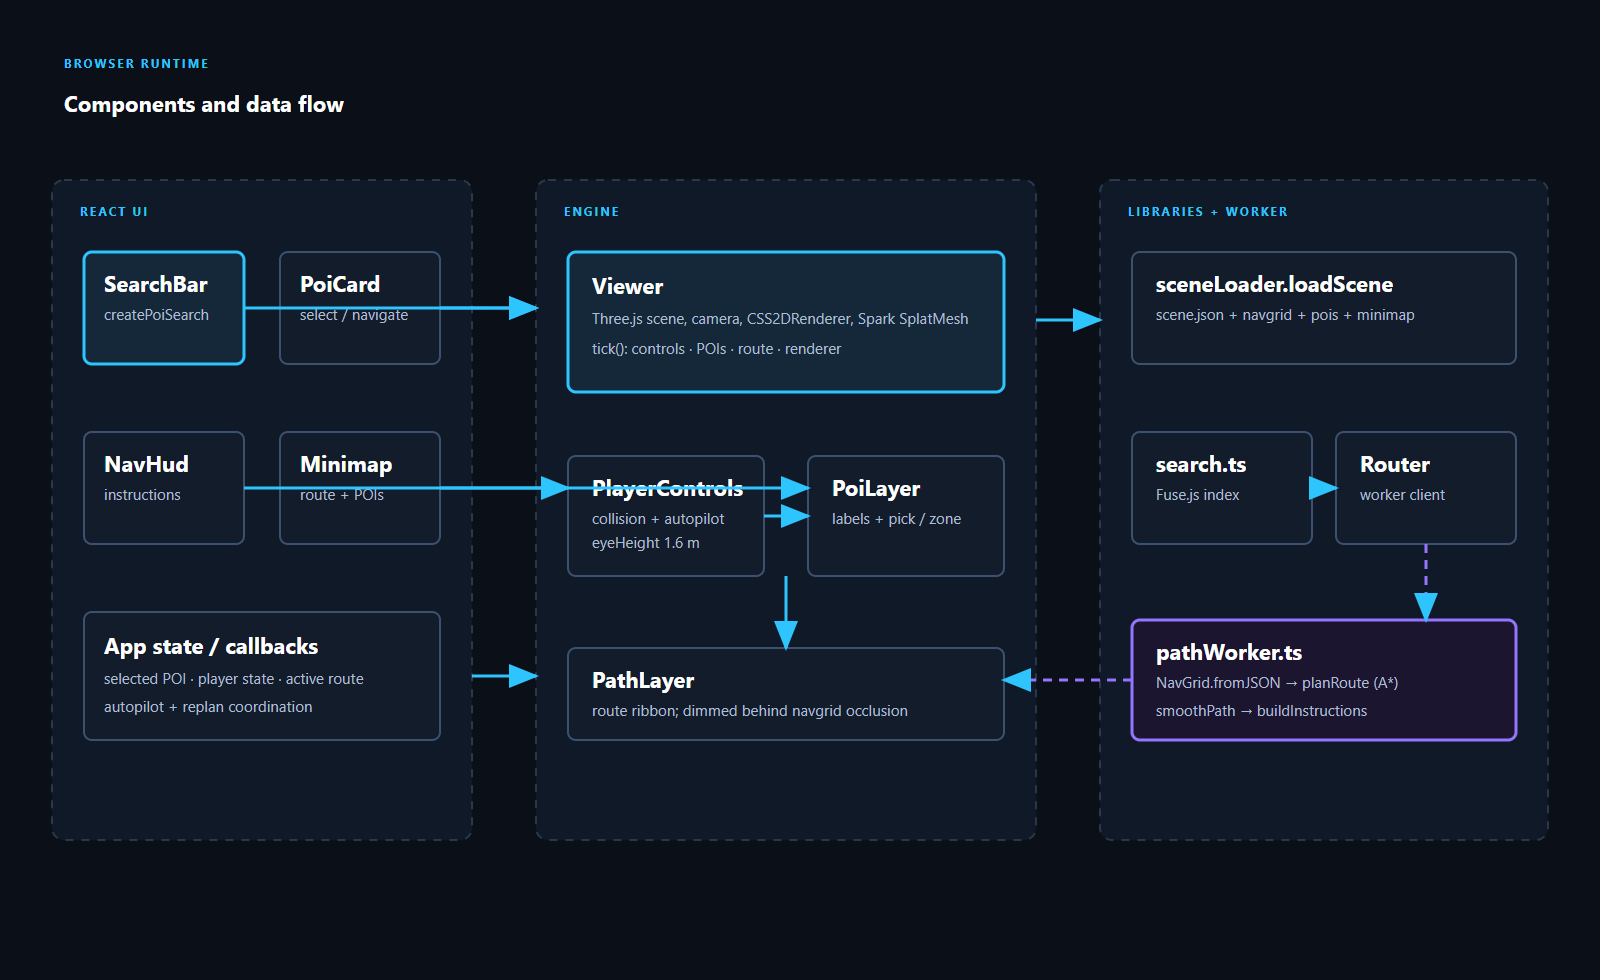
\includegraphics[width=0.92\textwidth]{figures/runtime-components.png}
\caption{Browser runtime components and data flow. The React user interface (search bar, place card, navigation HUD, minimap) talks to the engine (viewer, player controls, place and path layers), which uses the scene loader, the Fuse.js index, and a router that posts planning requests to the A* Web Worker.}
\label{fig:runtime}
\end{figure*}

\begin{figure}[!tb]
\centering
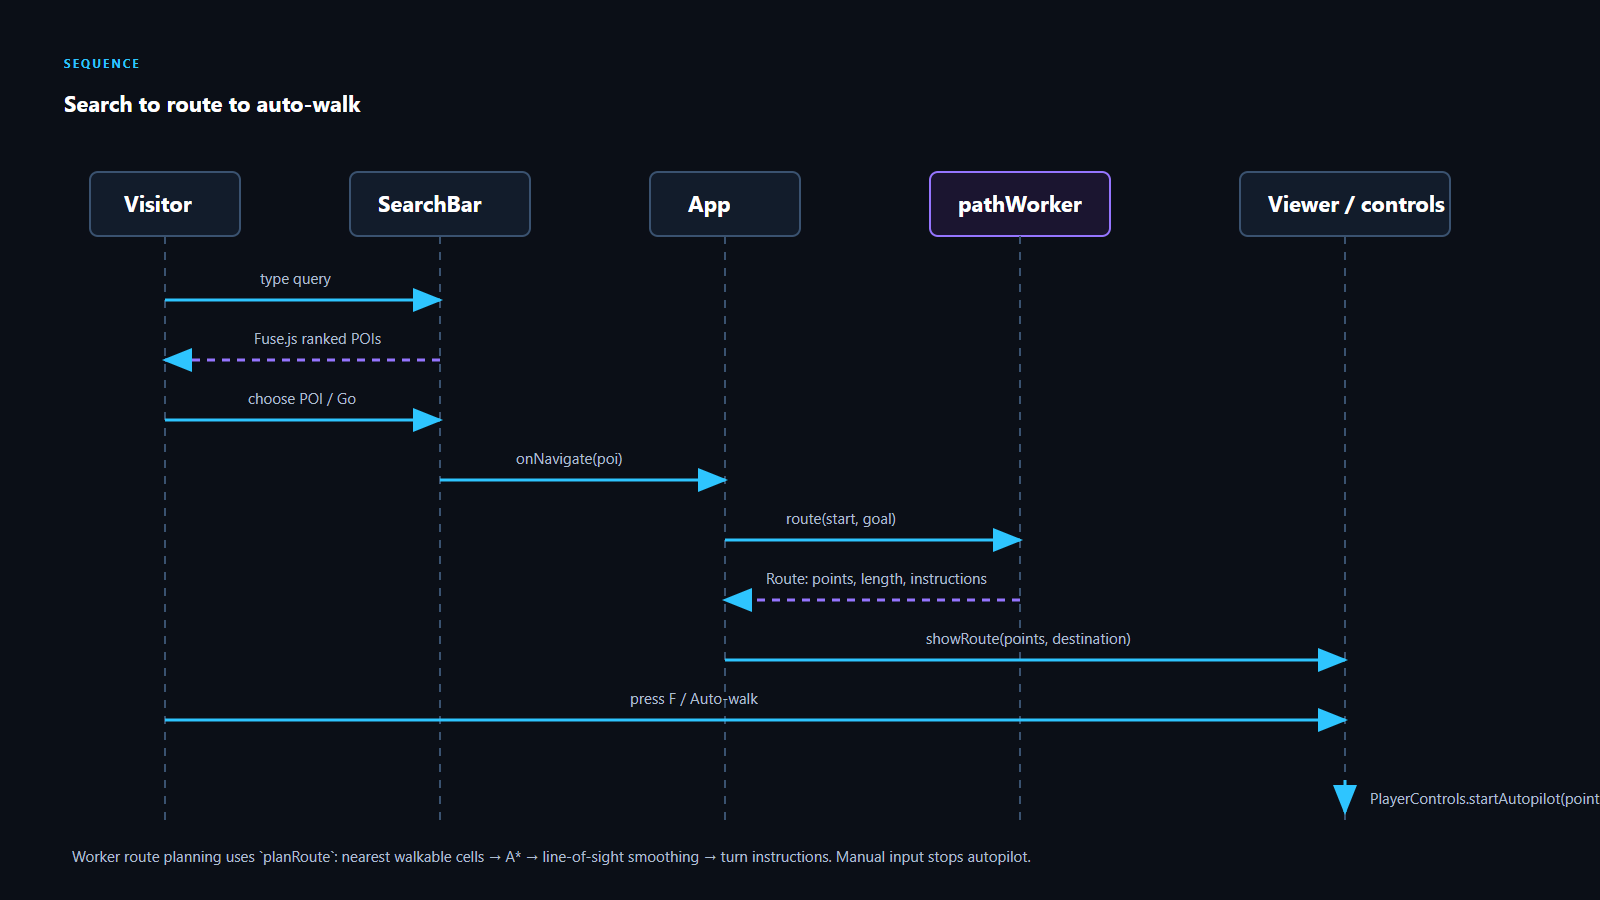
\includegraphics[width=\columnwidth]{figures/navigation-sequence.png}
\caption{Search-to-route-to-auto-walk sequence. A selected place triggers a plan request to the Web Worker, which returns points, length, and instructions for rendering; manual input stops auto-walk.}
\label{fig:nav_seq}
\end{figure}

\begin{table}[!htb]
\centering
\footnotesize
\caption{Point-of-Interest Record (\texttt{pois.json}, version 1)}
\label{tab:poi}
\begin{tabular}{p{0.20\columnwidth}p{0.17\columnwidth}p{0.45\columnwidth}}
\toprule
\textbf{Field} & \textbf{Type} & \textbf{Meaning} \\
\midrule
\texttt{id} & string & Stable key; deep link \texttt{?to=<id>} \\
\texttt{name} & string & Label and search text \\
\texttt{category} & string & One of nine; unknown falls back to \texttt{other} \\
\texttt{tags} & string[] & Optional search keywords \\
\texttt{description} & string & Optional free text \\
\texttt{position} & [x,y,z] & Label anchor in metric frame \\
\texttt{zone} & [[x,z],\ldots] & Optional floor polygon (3+ points) \\
\bottomrule
\end{tabular}
\end{table}

\subsection{Search}
Search builds a Fuse.js index \cite{fusejs} over places with field weights for \texttt{name} (0.6), \texttt{tags} (0.25), \texttt{category} (0.1), and \texttt{description} (0.05), a match threshold of 0.4 for typo tolerance, and \texttt{ignoreLocation} so a match anywhere in a string counts. The interface returns at most eight results; an empty query returns the first places unfiltered. Pressing \texttt{/} focuses the box, Enter jumps to a place, and Shift+Enter starts navigation. Matching is lexical, so synonyms exist only if authors add them as tags.

\subsection{Pathfinding and Instructions}
Routing runs A* \cite{hart1968astar} over the walkable cells of the grid, 8-connected, with diagonal cost $\sqrt{2}$ and no corner cutting: a diagonal step requires both adjacent orthogonal cells to be walkable. The cost of stepping into cell $v$ with base length $w_{uv}\in\{1,\sqrt{2}\}$ and clearance $\kappa(v)$ is
\begin{equation}
c(u\!\to\!v) = w_{uv}\left(1 + \lambda \max\!\left(0,\, 1 - \frac{\kappa(v)}{\kappa_0}\right)\right),
\end{equation}
with preferred clearance $\kappa_0 = 0.6$~m and wall penalty $\lambda = 2$. A route that hugs a wall therefore pays up to $3\times$ the distance, so paths centre themselves in corridors and doorways. The heuristic is octile distance in cells,
\begin{equation}
h(r,c) = \Delta_r + \Delta_c + (\sqrt{2}-2)\min(\Delta_r,\Delta_c),
\end{equation}
which does not overestimate because the penalty only increases step costs. The open set is a binary min-heap with typed-array scores. Start and goal snap to the nearest walkable cell, and for a zone place the goal is the zone centroid. The cell path is smoothed by string pulling: points are dropped while the straight segment between the anchor and a candidate stays on walkable cells (sampled every half cell). The route begins exactly at the user's position when that spot is walkable.

Planning runs in a Web Worker. The router posts the grid once and then sends plan requests, so planning never blocks rendering; if a worker cannot be created, planning runs inline. While following a route, if the player drifts more than 1.6~m from the polyline (at least 1.5~s since the last plan and not during auto-walk), the route is re-planned from the current position.

At each interior vertex the signed turn angle
\begin{equation}
\theta = \operatorname{atan2}\!\left(\mathbf{a}\times\mathbf{b},\ \mathbf{a}\cdot\mathbf{b}\right)
\end{equation}
between the incoming and outgoing headings $\mathbf{a}$ and $\mathbf{b}$ is classified: below 20$^{\circ}$ is straight (no instruction), 20$^{\circ}$--50$^{\circ}$ slight left or right, 50$^{\circ}$--135$^{\circ}$ left or right, and above 135$^{\circ}$ a U-turn. The instruction list is \emph{start}, the turns with their distance along the route, and \emph{arrive}. The HUD shows an arrow, text such as ``Turn left in 6 m'' (``now'' within 1.5~m), the remaining distance, and an ETA at 1.2~m/s; arrival triggers within 0.9~m of the end. Auto-walk (key \texttt{F}) drives the camera along the route. Figure~\ref{fig:nav_seq} shows the interaction from search to auto-walk.

\subsection{Configuration Summary}
Table~\ref{tab:model_config} collects the main parameters. Values marked with an asterisk differ in the reported runs from the defaults, as noted in the text.

\begin{table}[!htb]
\centering
\footnotesize
\caption{Parameter Summary (Defaults Unless Marked)}
\label{tab:model_config}
\begin{tabular}{p{0.46\columnwidth}p{0.43\columnwidth}}
\toprule
\textbf{Item} & \textbf{Value} \\
\midrule
Keyframe rate / long side & 2 per s / 1600 px (run: 5.5 per s, 1024 px*) \\
Blur floor & 35\% of median sharpness \\
Camera model; SIFT features & \texttt{SIMPLE\_RADIAL}; 8,192 max \\
Match window & 15 neighbours \\
ArUco dictionary; side & \texttt{DICT\_4X4\_50}; 0.15 m \\
Phone height & 1.35 m \\
Floor tilt limit & 10$^{\circ}$ \\
Trainer; steps; cap & gsplat MCMC; 30k; 1.5M (run: Brush 20k, 25k*) \\
Cleaning & $\alpha{<}0.05$; extent $>$1 m; $k{=}8$, $3\sigma$ \\
Grid; agent radius; band & 5 cm; 0.25 m; 0.12--1.9 m \\
A* clearance, penalty & 0.6 m, 2.0 \\
Re-route; arrival & 1.6 m drift; 0.9 m \\
Eye height; walk speed; ETA speed & 1.6 m; 1.6 m/s; 1.2 m/s \\
\bottomrule
\end{tabular}
\end{table}

\subsection{Evaluation Quantities}
We report only quantities the pipeline records. The registration ratio $\rho$ and mean reprojection error $\bar{e}$ measure SfM. The retention ratio after cleaning is
\begin{equation}
\eta = \frac{N_{\mathrm{out}}}{N_{\mathrm{in}}},
\end{equation}
the compressed-splat and grid sizes are in megabytes and kilobytes, and the walkable area is
\begin{equation}
A_{\mathrm{walk}} = |\mathcal{W}| \cdot \delta^{2},
\end{equation}
with $\delta = 0.05$~m the cell size. We do not report novel-view PSNR, SSIM, absolute scale error, route-length accuracy, or user-task times, because those were not measured.

\section{Experimental Results}
\label{sec:results}
\subsection{Single-Video Run}
Table~\ref{tab:sfm} reports the single-video reconstruction. Of 293 extracted keyframes, 65 registered ($\rho = 22\%$) in the largest of 7 sub-models, with 6,660 sparse points and a mean reprojection error of 0.52~px. SfM took about 155~s on CPU. The low registration ratio follows the capture conditions: a low-texture interior and fast pans meant most frames could not be linked to the main model. The consequence is a partial reconstruction of the room.

\begin{figure*}[!tb]
\centering
\begin{minipage}[t]{0.48\textwidth}
\centering
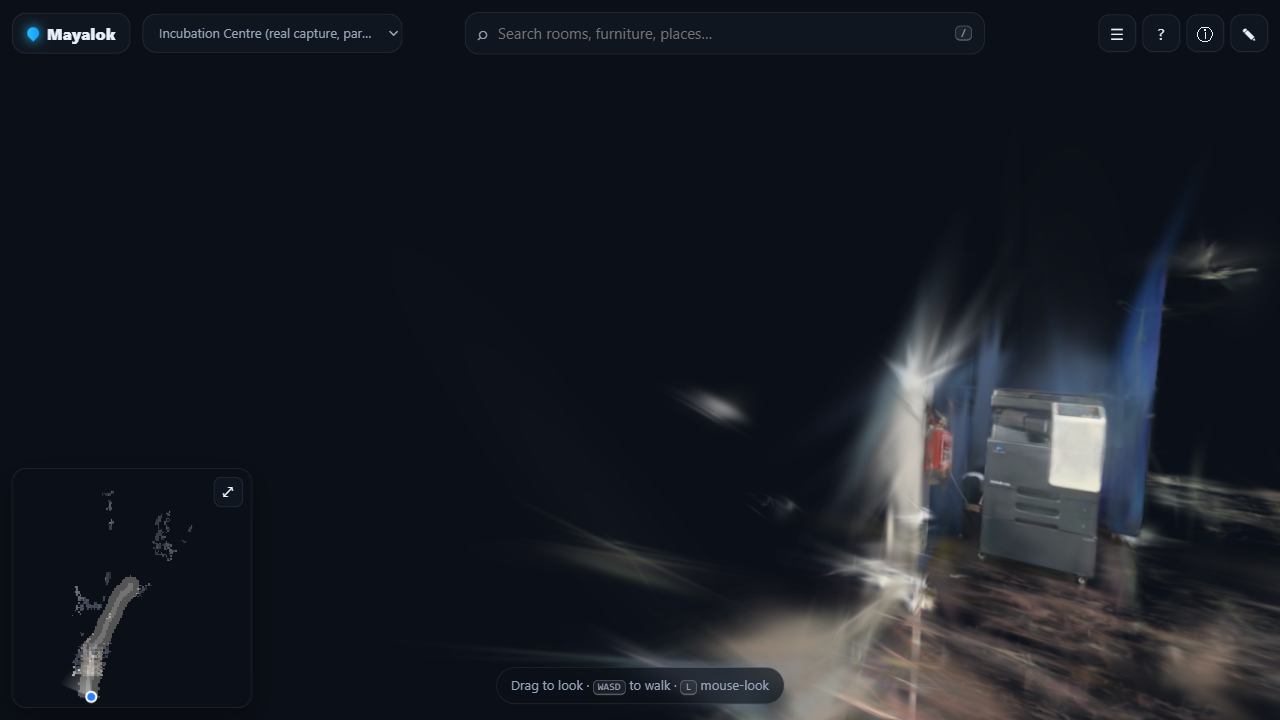
\includegraphics[width=\linewidth]{figures/shot-incubation.png}\\
{\footnotesize (a) Real capture: the incubation-centre scene from one phone video, with its minimap (65 of 293 keyframes registered).}
\end{minipage}
\hfill
\begin{minipage}[t]{0.48\textwidth}
\centering
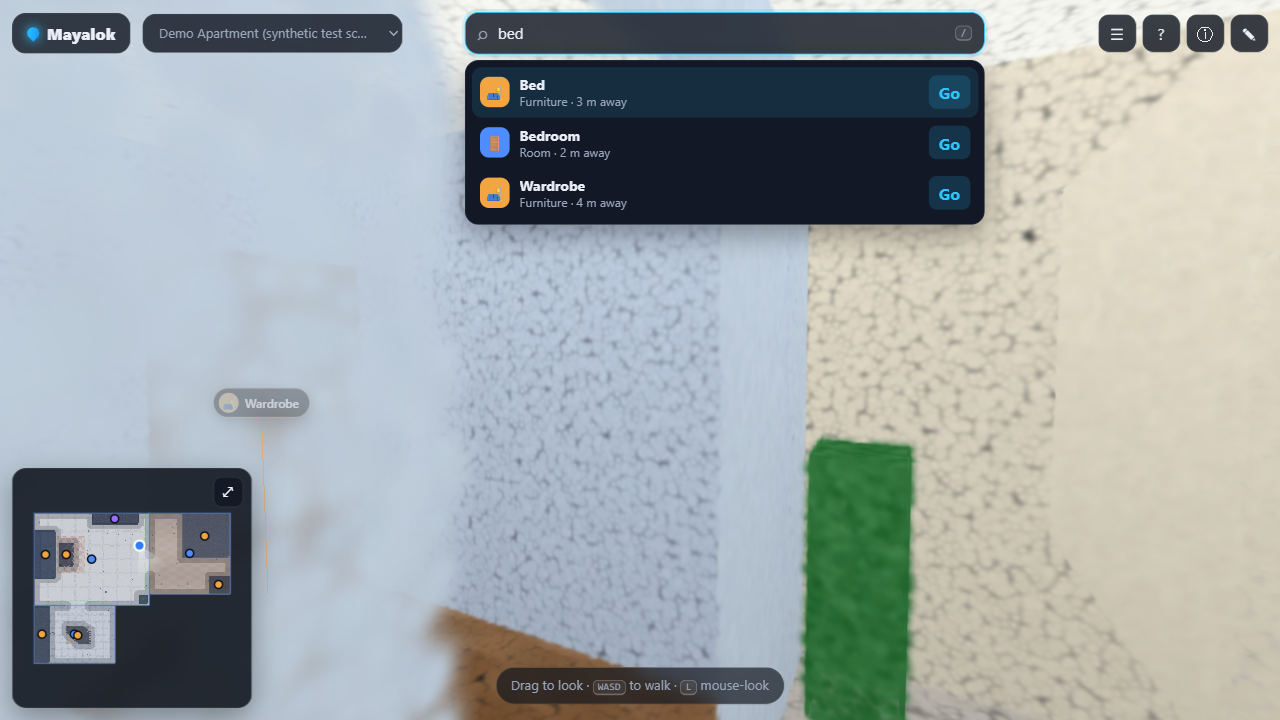
\includegraphics[width=\linewidth]{figures/shot-search.png}\\
{\footnotesize (b) Fuzzy search over tagged places on the synthetic \texttt{demo-apartment} scene, with category and live distance.}
\end{minipage}

\vspace{4pt}
\begin{minipage}[t]{0.48\textwidth}
\centering
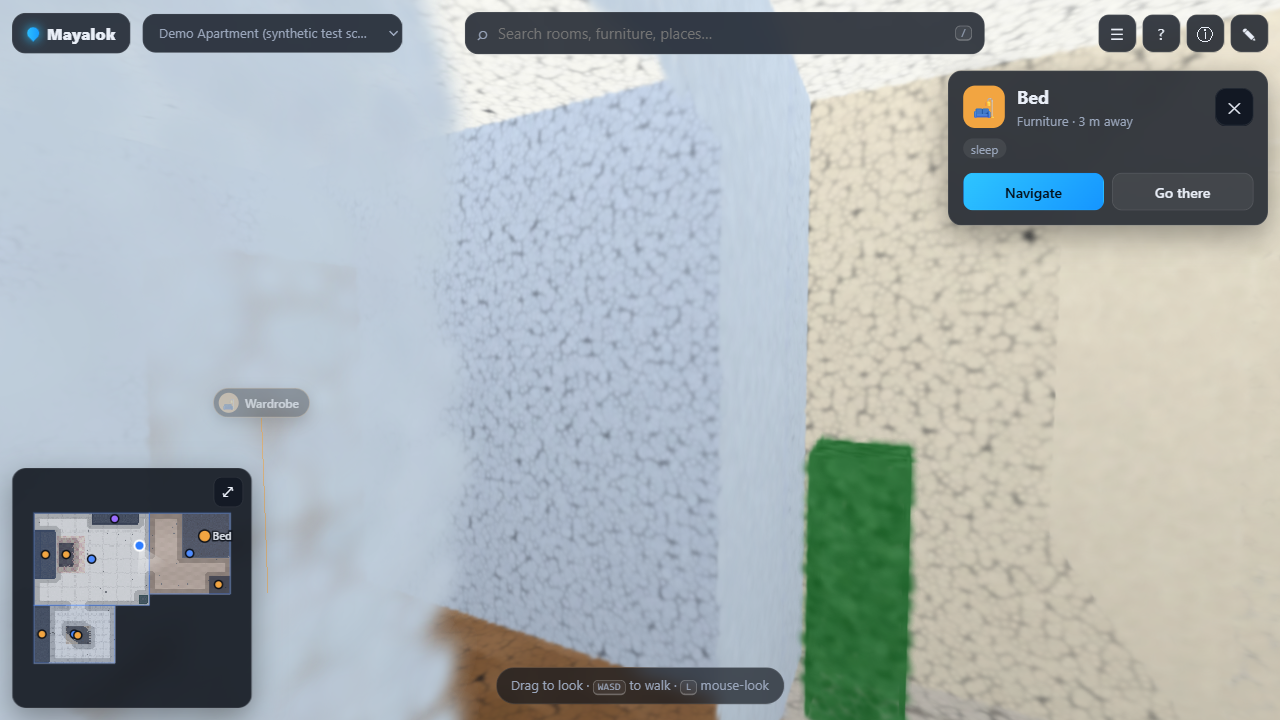
\includegraphics[width=\linewidth]{figures/shot-route.png}\\
{\footnotesize (c) Place card on the synthetic scene, offering Navigate and Go there.}
\end{minipage}
\hfill
\begin{minipage}[t]{0.48\textwidth}
\centering
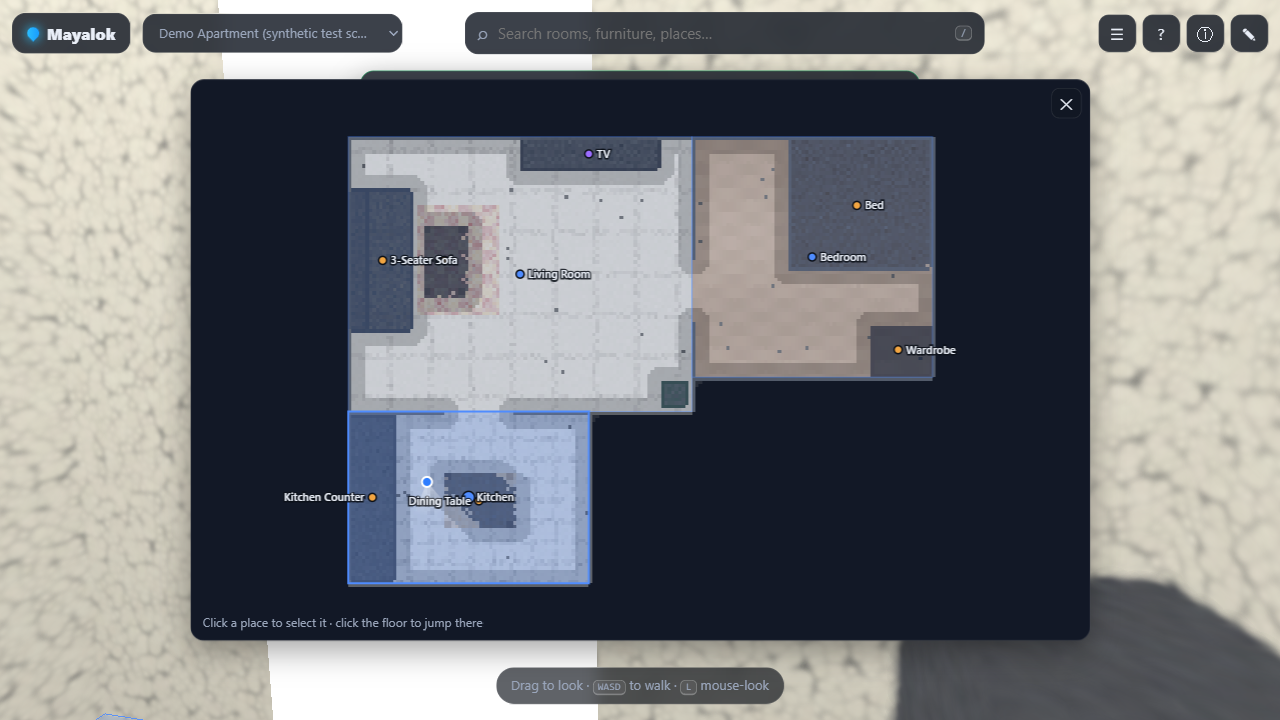
\includegraphics[width=\linewidth]{figures/shot-map.png}\\
{\footnotesize (d) Expanded floor map of the synthetic scene with room zones and tagged places.}
\end{minipage}
\caption{Viewer screenshots. Panel (a) is the real, partial reconstruction; panels (b)--(d) use the procedurally generated \texttt{demo-apartment} test scene and demonstrate interface features, not reconstruction quality.}
\label{fig:screens}
\end{figure*}

\begin{table}[!htb]
\centering
\footnotesize
\caption{Single-Video Run: SfM and Training}
\label{tab:sfm}
\begin{tabular}{p{0.52\columnwidth}r}
\toprule
\textbf{Quantity} & \textbf{Value} \\
\midrule
Input video (portrait) & 56.8 s \\
Keyframes extracted & 293 \\
Registered images (largest of 7 sub-models) & 65 \\
Registration ratio $\rho$ & 22\% \\
Sparse 3D points & 6,660 \\
Mean reprojection error $\bar{e}$ & 0.52 px \\
SfM wall time (CPU) & about 155 s \\
Trainer; steps & Brush; 20,000 \\
Raw Gaussians & 430,487 \\
\bottomrule
\end{tabular}
\end{table}

Brush trained 430,487 Gaussians for 20,000 steps on the laptop GPU. Table~\ref{tab:clean} breaks down the cleaning stage from \texttt{report.json}. About 51.5\% of the raw Gaussians were removed for low opacity, and a further 14,406 fell outside the bounds around the walked path; 191,378 remained, so $\eta = 44.5\%$. The floor refit applied a vertical shift of 0.285~m. The whole clean, grid, and export tail took 7.04~s.

\begin{table}[!htb]
\centering
\footnotesize
\caption{Single-Video Run: Cleaning, Grid, and Export (from \texttt{report.json})}
\label{tab:clean}
\begin{tabular}{p{0.52\columnwidth}r}
\toprule
\textbf{Quantity} & \textbf{Value} \\
\midrule
Input Gaussians & 430,487 \\
Removed, transparent ($\alpha<0.05$) & 221,679 \\
Removed, oversized & 230 \\
Removed, outside bounds & 14,406 \\
Removed, isolated (statistical) & 2,794 \\
Output Gaussians & 191,378 \\
Retention ratio $\eta$ & 44.5\% \\
Floor offset applied & 0.285 m \\
Grid size (rows $\times$ cols, 5 cm) & 140 $\times$ 95 \\
Obstacle cells; floor cells & 567; 138 \\
Walkable area, shipped grid & 2.66 m\textsuperscript{2} \\
Walkable area at 0.25 m radius & 0.71 m\textsuperscript{2} \\
\texttt{scene.spz} size & 4.7 MB \\
\texttt{navgrid.json} size & 35.7 KB \\
Clean / grid / export time & 0.86 s / 0.04 s / 6.14 s \\
\bottomrule
\end{tabular}
\end{table}

\subsection{Walkable Area and Agent Radius}
The shipped grid was built with a reduced agent radius of 0.05~m (the \texttt{agentRadius} field of \texttt{navgrid.json}), which gives $A_{\mathrm{walk}} = 2.66$~m\textsuperscript{2}. At the default 0.25~m the same scene yields only 0.71~m\textsuperscript{2}. The reason is visible in the construction. Only 138 floor cells (0.35~m\textsuperscript{2}) had reconstructed floor evidence, whereas the walkable set contains $2.66/0.05^{2} = 1{,}064$ cells, so most walkable cells come from the walked-path repair rule, which frees a 0.3~m radius around the camera trajectory. That makes the free region a narrow strip, and inflating obstacles by 0.25~m leaves little of it. We therefore treat the 2.66~m\textsuperscript{2} grid as a tuned setting that keeps routes possible in a partial scene, not as evidence of a fully mapped room, and the radius is a build-time parameter with no runtime override in the viewer. The scene is a corridor-like fragment, as the minimap in Fig.~\ref{fig:screens}(a) shows.

\subsection{All-Captures Run}
We also ran the pipeline on all 603 images (7 videos and 32 photos) of the same venue. Table~\ref{tab:compare} compares the two runs. GLOMAP registered 523 of 603 images (86.7\%) in a single model, and 496 remained after outlier removal, with a mean reprojection error of 0.72~px. Brush trained 520,066 Gaussians for 25,000 steps. Judged on registration ratio and reprojection error, this run looks better than the single-video run. Visually it failed: the splat showed cross-clip misalignment, that is, content from different clips did not line up, and we excluded it from the shipped scene. The single-video scene is therefore the one packaged with the viewer.

\begin{table}[!htb]
\centering
\footnotesize
\caption{Comparison of the Two Reconstruction Runs}
\label{tab:compare}
\resizebox{\columnwidth}{!}{%
\begin{tabular}{p{0.34\columnwidth}p{0.30\columnwidth}p{0.30\columnwidth}}
\toprule
\textbf{Item} & \textbf{Single video} & \textbf{All captures} \\
\midrule
Images & 293 keyframes & 603 \\
SfM engine & pycolmap, 7 sub-models & GLOMAP, one model \\
Registered & 65 (22\%) & 523 (86.7\%); 496 after outlier removal \\
Mean reprojection error & 0.52 px & 0.72 px \\
Sparse points & 6,660 & not recorded here \\
Trainer; steps & Brush; 20k & Brush; 25k \\
Gaussians & 430,487 raw; 191,378 clean & 520,066 \\
Outcome & Packaged as \texttt{incubation} scene & Visual cross-clip misalignment; excluded \\
\bottomrule
\end{tabular}%
}
\end{table}

\subsection{Why Reprojection Error Did Not Predict Usability}
The all-captures run is the most instructive result. Mean reprojection error is a local residual: it is small when each point projects close to its measured keypoint in the images that observe it. It does not constrain whether two clips that never share many observations are placed consistently. Registering 523 images into one model at 0.72~px can therefore coexist with a pair of clips offset from each other. We did not isolate the cause. Plausible, untested factors in this configuration are (i) separate intrinsics per clip, (ii) sequential matching, which links frames mainly within a clip and across clip boundaries only through neighbours in file order unless the optional vocabulary tree is enabled, and (iii) repetitive or low-texture surfaces that produce wrong cross-clip matches. These are hypotheses to test with a loop-closure matcher and ArUco markers visible in several clips, not findings. The practical lesson, which feeds the revised SOP, is to check a splat visually, and ideally against held-out views, before trusting registration statistics.

\subsection{Viewer Output}
Figure~\ref{fig:screens}(a) shows the real incubation scene in the viewer, with the minimap in the lower left. The reconstruction is partial: a printer, a red object, and a blue partition are recognizable, while surrounding regions are dark or stretched into streaks where Gaussians are poorly constrained. Figures~\ref{fig:screens}(b)--(d) show search, the place card, and the floor map on the \texttt{demo-apartment} scene, a procedurally generated three-room apartment used for development and tests. These three screenshots demonstrate the interface and routing features on synthetic data, not reconstruction quality; the \texttt{incubation} scene currently ships with an empty \texttt{pois.json}, so its places are still to be annotated.

\subsection{Software Verification}
The routing library has 11 passing unit tests (vitest, \texttt{astar.test.ts}) covering the A* search, turn instructions, and polygon geometry, and the pipeline has a pytest suite (alignment, navigation grid, SfM, splats and frames) that runs offline on a synthetic apartment generator. We do not quote coverage figures. Planning time in milliseconds is returned with each route and logged to the console, but we have no benchmark table for it, so we make no latency claim. The reconstruction pipeline is published as the \texttt{mayalok} package (\texttt{pip install mayalok}, PyPI 0.1.0).

\FloatBarrier

\section{Discussion}
The results support a focused claim. A single handheld smartphone video can produce, with about 155~s of CPU SfM and a Brush training run on a laptop GPU, a compact splat (4.7~MB) and a derived grid that the viewer can render and route over. The same evidence also shows the limits of that claim: only 22\% of keyframes registered, the reconstruction covers part of one room, and metric scale rests on an assumed phone height rather than printed markers. The distances, route lengths, and ETAs the viewer reports are therefore only as accurate as that assumption.

The single-grid design has a practical advantage and a cost. Because collision, routing, line-of-sight dimming of labels and route ribbons, and the minimap all read the same grid, they are consistent with each other and cheap to compute in the browser. The cost is that obstacles come from splat density, so thin or transparent objects, glass, and mirrors can be missed or ghosted, and the grid is two-dimensional. The walked-path repair rule also trades safety for completeness: it keeps routes available in a texture-poor floor, but it can mark as free a cell the camera passed over without ever observing the floor there.

The failed all-captures run is a more useful outcome than a clean success would have been. It shows that a pipeline whose summary statistics look good can still emit an unusable splat, which is why each scene ships its build statistics in \texttt{report.json} and why the revised SOP asks for slower pans, more overlap, and printed markers. We do not claim the 523-image result is wrong, only that it was visually unusable for our purpose.

\section{Threats to Validity}
\textbf{Single venue and single run per configuration.} All numbers come from one capture session. We cannot say how registration, cleaning, or grid statistics vary across venues, lighting, or phones, and we report no confidence intervals.

\textbf{Metric scale.} Scale for the shipped scene comes from the 1.35~m phone-height rule, not ArUco markers, and we did not measure a ground-truth distance in the venue. The scale error is unknown.

\textbf{No image-quality metrics.} Held-out PSNR and SSIM were not recorded for either run, and visual assessment of the failed run is qualitative.

\textbf{Tuned grid.} The shipped walkable area uses a 0.05~m agent radius rather than the 0.25~m default, and most walkable cells come from the walked-path repair rule. The grid should not be read as an independent measurement of free floor.

\textbf{No user study or latency benchmark.} We did not test the viewer with users, and we did not tabulate planning time or frame rate.

\textbf{Synthetic demonstrations.} The search, place-card, and map screenshots use a procedurally generated scene. They show interface behavior, not reconstruction fidelity.

\textbf{Documentation drift.} Some project documents describe defaults (30,000 steps, gsplat) that differ from the settings used in the reported runs (Brush, 20,000 and 25,000 steps). We report the run settings.

\section{Limitations and Future Work}
\textbf{Known limitations.} The grid is single-floor, so stairs, ramps, and multi-level venues are not modelled. Dynamic obstacles (people, moved furniture) are not detected. Splats carry no explicit surface mesh. Mirrors, glass, and blank walls degrade SfM and training, and training needs a CUDA GPU (a cloud notebook is the fallback). Search is lexical. Admin edits are browser-local until exported. There is no multi-user editing.

\textbf{Near-term work.} The immediate extension is a re-capture of the incubation centre that follows the revised SOP, with printed ArUco markers visible in several clips and vocabulary-tree loop detection enabled, to test the hypotheses in Section~\ref{sec:results}. We would then record held-out PSNR and SSIM, measure a known distance to quantify scale error, and tabulate planning latency.

\textbf{Longer-term work.} The planned augmented-reality layer would localize a phone camera against the splat and overlay the route on the live camera feed, using the floor markers already exported as anchors in \texttt{scene.json}. Further directions are semi-automatic place suggestion from the splat, incremental re-capture of changed zones, and multi-floor stitching.

\section{Conclusion}
This report presents Mayalok, a pipeline and static web viewer that turns smartphone video into a metric Gaussian-splat digital twin with a 5~cm walkable grid, fuzzy place search, and wall-aware A* routing in the browser. On one real incubation-centre capture, a single 56.8~s video produced 65 registered keyframes out of 293, a 191,378-Gaussian cleaned splat, a 4.7~MB \texttt{scene.spz}, and a 2.66~m\textsuperscript{2} walkable area after agent-radius tuning (0.71~m\textsuperscript{2} at 0.25~m). A 603-image run registered 523 images at 0.72~px yet failed visually and was excluded, showing that registration statistics alone do not certify a usable splat. The main value of this version is clarity about what is demonstrated, a working end-to-end system with a partial real scene, and what remains to be validated, namely scale accuracy, image quality, multi-clip consistency, and user-facing performance.

\section*{Acknowledgment}
The authors thank the open-source communities behind COLMAP and GLOMAP, gsplat, Brush, Three.js, Spark.js, Fuse.js, and splat-transform, whose tools made this system possible, and the Techfest 2026--27 Namma Space challenge organizers at IIT Bombay.

\FloatBarrier
\bibliographystyle{IEEEtran}
\bibliography{references}

\end{document}
